\documentclass{article}
\usepackage[spanish]{babel}
\usepackage[utf8]{inputenc}
\usepackage{longtable}
\usepackage{array}
\usepackage{graphicx}
\usepackage{listings}
\usepackage{xcolor}

\title{Inteligencia Artificial: Formulación, análisis e implementación en Lisp-Scheme del problema "Misioneros y Caníbales"}
\author{Carlos Javier Tacón Fernández} 
\date{\today}

\begin{document}

\pagenumbering{gobble}
\begin{titlepage}
  \thispagestyle{empty}
  \maketitle
\end{titlepage}
\pagenumbering{arabic}

\tableofcontents
\pagebreak

\section{MC-1}
Versión clásica del problema: encontrar con qué movimientos pueden atravesar un río tres misioneros y tres caníbales utilizando una barca de dos plazas, que al menos debe llevar un pasajero para remar, partiendo todos de una de las orillas y con la condición de que en ningún momento queden en ninguna de las orillas más caníbales que misioneros.

\subsection{Formulación del problema}
\begin{itemize}
  \item \textbf{Morfología de un estado:} \{Nº misioneros orilla izquierda, Nº caníbales orilla izquierda, Nº misioneros orilla derecha, Nº caníbales orilla derecha\}. El estado será válido si no hay más caníbales que misioneros en cada una de las orillas, a no ser que haya solamente caníbales. Solo se contemplarán números naturales y la suma de elementos entre las dos orillas será constante (3 misioneros y 3 caníbales).
  \item \textbf{Estado inicial:} \{0, 0, 3, 3\}.
  \item \textbf{Estado meta:} \{3, 3, 0, 0\}.
  \item \textbf{Estados disponibles:} \{0, 0, 3, 3\}, \{0, 1, 3, 2\}, \{0, 2, 3, 1\}, \{0, 3, 3, 0\}, \{1, 1, 2, 2\}, \{2, 2, 1, 1\}, \{3, 0, 0, 3\}, \{3, 1, 0, 2\}, \{3, 2, 0, 1\}, \{3, 3, 0, 0\}.
  \item \textbf{Coste de las operaciones:} Suponemos que todas las operaciones tienen igual coste (1).
  \item \textbf{Operaciones disponibles:} Las operaciones serán hacia una orilla u otra dependiendo de dónde se encuentre la barca. Para ello utilizaremos la paridad de la profundidad del nodo a evaluar. La barca tiene máximo dos plazas pero siempre tendrá que haber una persona para dirigirla.
  \begin{enumerate}
    \item Mover un misionero.
    \item Mover dos misioneros.
    \item Mover un caníbal.
    \item Mover dos caníbales.
    \item Mover un misionero y un caníbal.
  \end{enumerate}
\end{itemize}

\subsection{Análisis de la solución}
El problema puede resolverse mediante búsqueda desinformada, por los métodos de búsqueda en anchura, búsqueda en profundidad iterativa o búsqueda bidireccional. También podríamos pensar alguna heurística válida, como por ejemplo, si el objetivo es que todas las personas lleguen a la orilla izquierda, podrían tener más preferencia los estados donde haya más personas en esa orilla (\{3, 0, 0, 3\} mejor que \{1, 1, 2, 2\}) así podríamos intentar utilizar el método de búsqueda primero el mejor.

Para mejorar la eficiencia del algoritmo podemos guardar una lista de nodos cerrados, ya evaluados teniendo en cuenta el sentido de la operación, en este caso la paridad de la profundidad. También podemos hacer la implementación de tal manera que se descarten los estados generados inválidos (o ya evaluados anteriormente) para que no tengan que ser evaluados otra vez, ya que generarán los mismos descendientes y aumentará tanto el tiempo de procesamiento como la memoria necesaria para guardar la lista de abiertos.\\

Desarrollamos el árbol de expansión realizando búsqueda en anchura, gestionando la lista de abiertos como FIFO, además no generamos estados inválidos, y no añadimos duplicados a la lista de abiertos. Tampoco desarrollamos los estados que ya hemos evaluado anteriormente [....] (teniendo en cuenta el sentido del viaje, o lo que es lo mismo, la paridad de la profundidad del nodo en el árbol). Las operaciones para generar los hijos se marcan con ''Nº operación)'' y la profundidad del nodo con [profundidad]. \\

\begin{center}
  \begin{longtable}{ |p{2cm}|p{2cm}|>{\raggedright\arraybackslash}p{7cm}|  }
    \hline
    Estado actual & Hijos & Abiertos \\ [0.5ex] 
    \hline\hline
    
    - & - & [0]\{0,0,3,3\} \\ 
    \hline
    [0]\{0,0,3,3\} & 3)[1]\{0,1,3,2\}, 4)[1]\{0,2,3,1\}, 5)[1]\{1,1,2,2\} & [1]\{0,1,3,2\}, [1]\{0,2,3,1\}, [1]\{1,1,2,2\} \\ 
    \hline
    [1]\{0,1,3,2\} & 3)[2]\{0,0,3,3\} & [1]\{0,2,3,1\}, [1]\{1,1,2,2\}, [2]\{0,0,3,3\} \\ 
    \hline
    [1]\{0,2,3,1\} & 3)[2]\{0,1,3,2\}, 4)[2]\{0,0,3,3\} & [1]\{1,1,2,2\}, [2]\{0,0,3,3\}, [2]\{0,1,3,2\} \\ 
    \hline
    [1]\{1,1,2,2\} & 1)[2]\{0,1,3,2\}, 5)[2]\{0,0,3,3\} & [2]\{0,0,3,3\}, [2]\{0,1,3,2\} \\ 
    \hline
    [2]\{0,0,3,3\} & .... & [2]\{0,1,3,2\} \\ 
    \hline
    [2]\{0,1,3,2\} & 1)[3]\{1,1,2,2\}, 3)[3]\{0,2,3,1\}, 4)[3]\{0,3,3,0\} & [3]\{1,1,2,2\}, [3]\{0,2,3,1\}, [3]\{0,3,3,0\} \\ 
    \hline
    [3]\{1,1,2,2\} & .... & [3]\{0,2,3,1\}, [3]\{0,3,3,0\} \\ 
    \hline
    [3]\{0,2,3,1\} & .... & [3]\{0,3,3,0\} \\ 
    \hline
    [3]\{0,3,3,0\} & 3)[4]\{0,2,3,1\}, 4)[4]\{0,1,3,2\} & [4]\{0,2,3,1\}, [4]\{0,1,3,2\} \\ 
    \hline
    [4]\{0,2,3,1\} & 2)[5]\{2,2,1,1\}, 4)[5]\{0,3,3,0\} & [4]\{0,1,3,2\}, [5]\{2,2,1,1\}, [5]\{0,3,3,0\} \\ 
    \hline
    [4]\{0,1,3,2\} & .... & [5]\{2,2,1,1\}, [5]\{0,3,3,0\} \\ 
    \hline
    [5]\{2,2,1,1\} & 2)[6]\{0,2,3,1\}, 5)[6]\{1,1,2,2\} & [5]\{0,3,3,0\}, [6]\{0,2,3,1\}, [6]\{1,1,2,2\} \\ 
    \hline
    [5]\{0,3,3,0\} & .... & [6]\{0,2,3,1\}, [6]\{1,1,2,2\} \\ 
    \hline
    [6]\{0,2,3,1\} & .... & [6]\{1,1,2,2\} \\ 
    \hline
    [6]\{1,1,2,2\} & 2)[7]\{3,1,0,2\}, 5)[7]\{2,2,1,1\} & [7]\{3,1,0,2\}, [7]\{2,2,1,1\} \\ 
    \hline
    [7]\{3,1,0,2\} & 2)[8]\{1,1,2,2\}, 3)[8]\{3,0,0,3\} & [7]\{2,2,1,1\}, [8]\{1,1,2,2\}, [8]\{3,0,0,3\} \\ 
    \hline
    [7]\{2,2,1,1\} & .... & [8]\{1,1,2,2\}, [8]\{3,0,0,3\} \\ 
    \hline
    [8]\{1,1,2,2\} & .... & [8]\{3,0,0,3\} \\ 
    \hline
    [8]\{3,0,0,3\} & 3)[9]\{3,1,0,2\}, 4)[9]\{3,2,0,1\} & [9]\{3,1,0,2\}, [9]\{3,2,0,1\} \\ 
    \hline
    [9]\{3,1,0,2\} & .... & [9]\{3,2,0,1\} \\ 
    \hline
    [9]\{3,2,0,1\} & 1)[10]\{2,2,1,1\}, 3)[10]\{3,1,0,2\}, 4)[10]\{3,0,0,3\} & [10]\{2,2,1,1\}, [10]\{3,1,0,2\}, [10]\{3,0,0,3\} \\ 
    \hline
    [10]\{2,2,1,1\} & 1)[11]\{3,2,0,1\}, 5)[11]\{3,3,0,0\} & [10]\{3,1,0,2\}, [10]\{3,0,0,3\}, [11]\{3,2,0,1\}, [11]\{3,3,0,0\} \\ 
    \hline
    [10]\{3,1,0,2\} & 3)[11]\{3,2,0,1\}, 4)[11]\{3,3,0,0\} & [10]\{3,0,0,3\}, [11]\{3,2,0,1\}, [11]\{3,3,0,0\} \\ 
    \hline
    [10]\{3,0,0,3\} & .... & [11]\{3,2,0,1\}, [11]\{3,3,0,0\} \\ 
    \hline
    [11]\{3,2,0,1\} & .... & [11]\{3,3,0,0\} \\ 
    \hline
    [11]\{3,3,0,0\} & Éxito & - \\ 
    \hline
  \end{longtable}
\end{center}

El programa implementado en Lisp-Scheme Racket (Anexo A) ha sido escrito usando el algoritmo de búsqueda en anchura, sin generar nodos que sean inválidos. No se ha tenido en cuenta ninguna lista de nodos cerrados, tampoco se ha tenido en cuenta evitar añadir a abiertos nodos con estados duplicados ni se ha implementado una heurística válida. Esto no impide encontrar la respuesta al problema pero el programa consumirá más tiempo y memoria. Al ejecutar el programa podemos ver la respuesta que imprime y el tiempo que ha tardado en encontrarla. La misma respuesta que hemos encontrado con el procedimiento manual. \\

\pagebreak
En un principio se hizo una implementación que generaba todos los nodos a partir de las operaciones sin tener en cuenta su validez. Se puede ver el resultado en la siguiente imagen. \\
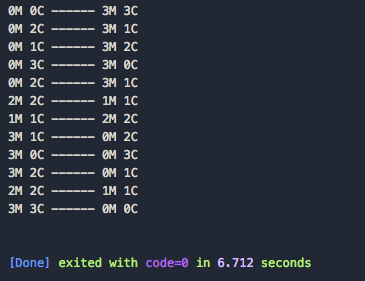
\includegraphics[width=8cm]{resources/mc-1} \\

Para intentar mejorar este tiempo de ejecución se implementó una manera de generación de descendientes que solo genera los descendientes que a priori son válidos. Con ese cambio se ha conseguido una mejora notable en el tiempo de ejecución final.\\
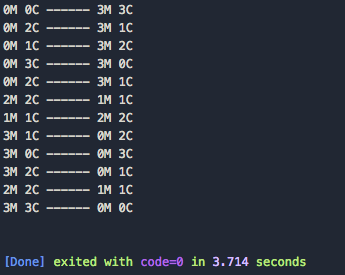
\includegraphics[width=8cm]{resources/mc-1v2} \\


\pagebreak
\section{MC-2}
Versión modificada del problema: encontrar con qué movimientos pueden atravesar un río cuatro misioneros y cuatro caníbales utilizando una barca de dos plazas, que al menos debe llevar un pasajero para remar, partiendo todos de una de las orillas y con la condición de que en ningún momento queden en ninguna de las orillas más caníbales que misioneros.

\subsection{Formulación del problema}
\begin{itemize}
  \item \textbf{Morfología de un estado:} \{Nº misioneros orilla izquierda, Nº caníbales orilla izquierda, Nº misioneros orilla derecha, Nº caníbales orilla derecha\}. El estado será válido si no hay más caníbales que misioneros en cada una de las orillas, a no ser que haya solamente caníbales. Solo se contemplarán números naturales y la suma de elementos entre las dos orillas será constante (4 misioneros y 4 caníbales).
  \item \textbf{Estado inicial:} \{0, 0, 4, 4\}.
  \item \textbf{Estado meta:} \{4, 4, 0, 0\}.
  \item \textbf{Estados disponibles:} \{0, 0, 4, 4\}, \{0, 1, 4, 3\}, \{0, 2, 4, 2\}, \{0, 3, 4, 1\}, \{0, 4, 4, 0\}, \{1, 1, 3, 3\}, \{2, 2, 2, 2\}, \{3, 3, 1, 1\}, \{4, 0, 0, 4\}, \{4, 1, 0, 3\}, \{4, 2, 0, 2\}, \{4, 3, 0, 1\}, \{4, 4, 0, 0\}.
  \item \textbf{Coste de las operaciones:} Suponemos que todas las operaciones tienen igual coste (1).
  \item \textbf{Operaciones disponibles:} Las operaciones serán hacia una orilla u otra dependiendo de dónde se encuentre la barca. Para ello utilizaremos la paridad de la profundidad del nodo a evaluar. La barca tiene máximo dos plazas pero siempre tendrá que haber una persona para dirigirla.
  \begin{enumerate}
    \item Mover un misionero.
    \item Mover dos misioneros.
    \item Mover un caníbal.
    \item Mover dos caníbales.
    \item Mover un misionero y un caníbal.
  \end{enumerate}
\end{itemize}

\subsection{Análisis de la solución}
Podemos observar que en esta versión del problema, al cambiar el número de misioneros y caníbales, obtenemos un espacio de estados posibles diferente, más amplio, además de cambiar el estado inicial y final. Las operaciones se mantienen exactamente igual que en el apartado anterior, ya que la capacidad de la barca se mantiene en 2.\\

Este problema no tiene solución, no se puede encontrar un camino para que todas las personas pasen de un lado a otro del río sin que los caníbales se coman a los misioneros ya que la limitación de la barca a 2 personas hace que, llagado un punto, no podamos avanzar en el espacio de estados. Vamos a observar qué pasa si intentamos desarrollar el árbol de expansión por el método de búsqueda en anchura, al igual que anteriormente, sin añadir duplicados a la lista de abiertos y sin desarrollar estados que ya hemos evaluado anteriormente [....] (teniendo en cuenta el sentido del viaje, o lo que es lo mismo, la paridad de la profundidad del nodo en el árbol). \\

\begin{center}
  \begin{longtable}{ |p{2cm}|p{2cm}|>{\raggedright\arraybackslash}p{7cm}|  }
    \hline
    Estado actual & Hijos & Abiertos \\ [0.5ex] 
    \hline\hline
    
    - & - & [0]\{0,0,4,4\} \\ 
    \hline
    [0]\{0,0,4,4\} & 3)[1]\{0,1,4,3\}, 4)[1]\{0,2,4,2\}, 5)[1]\{1,1,3,3\} & [1]\{0,1,4,3\}, [1]\{0,2,4,2\}, [1]\{1,1,3,3\}  \\ 
    \hline
    [1]\{0,1,4,3\} & 3)[2]\{0,0,4,4\} & [1]\{0,2,4,2\}, [1]\{1,1,3,3\}, [2]\{0,0,4,4\} \\ 
    \hline   
    [1]\{0,2,4,2\} & 3)[2]\{0,1,4,3\}, 4)[2]\{0,0,4,4\} & [1]\{1,1,3,3\}, [2]\{0,0,4,4\}, [2]\{0,1,4,3\} \\ 
    \hline
    [1]\{1,1,3,3\} & 1)[2]\{0,1,4,3\}, 5)[2]\{0,0,4,4\} & [2]\{0,0,4,4\}, [2]\{0,1,4,3\} \\ 
    \hline
    [2]\{0,0,4,4\} & .... & [2]\{0,1,4,3\} \\ 
    \hline
    [2]\{0,1,4,3\} & 1)[3]\{1,1,3,3\}, 3)[3]\{0,2,4,2\}, 4)[3]\{0,3,4,1\} & [3]\{1,1,3,3\}, [3]\{0,2,4,2\}, [3]\{0,3,4,1\} \\ 
    \hline
    [3]\{1,1,3,3\} & .... & [3]\{0,2,4,2\}, [3]\{0,3,4,1\} \\ 
    \hline
    [3]\{0,2,4,2\} & .... & [3]\{0,3,4,1\} \\ 
    \hline
    [3]\{0,3,4,1\} & 3)[4]\{0,2,4,2\}, 4)[4]\{0,1,4,3\} & [4]\{0,2,4,2\} \\ 
    \hline
    [4]\{0,2,4,2\} & 2)[5]\{2,2,2,2\}, 3)[5]\{0,3,4,1\}, 4)[5]\{0,4,4,0\} & [5]\{2,2,2,2\}, [5]\{0,3,4,1\}, [5]\{0,4,4,0\} \\ 
    \hline
    [4]\{2,2,2,2\} & 2)[6]\{0,2,4,2\}, 5)[6]\{1,1,3,3\} & [5]\{0,3,4,1\}, [5]\{0,4,4,0\}, [6]\{0,2,4,2\}, [6]\{1,1,3,3\} \\ 
    \hline
    [5]\{0,3,4,1\} & .... & [5]\{0,4,4,0\}, [6]\{0,2,4,2\}, [6]\{1,1,3,3\} \\ 
    \hline
    [5]\{0,4,4,0\} & 3)[6]\{0,3,4,1\}, 4)[6]\{0,2,4,2\} & [6]\{0,2,4,2\}, [6]\{1,1,3,3\}, [6]\{0,3,4,1\} \\ 
    \hline
    [6]\{0,2,4,2\} & .... & [6]\{1,1,3,3\}, [6]\{0,3,4,1\} \\ 
    \hline
    [6]\{1,1,3,3\} & 5)[7]\{2,2,2,2\} & [6]\{0,3,4,1\}, [7]\{2,2,2,2\} \\ 
    \hline
    [6]\{0,3,4,1\} & 3)[7]\{0,4,4,0\} & [7]\{2,2,2,2\}, [7]\{0,4,4,0\} \\ 
    \hline
    [7]\{2,2,2,2\} & 5)[8]\{1,1,3,3\} & [7]\{0,4,4,0\}, [8]\{1,1,3,3\} \\ 
    \hline
    [7]\{0,4,4,0\} & .... & [8]\{1,1,3,3\} \\ 
    \hline
    [8]\{1,1,3,3\} & .... & .... \\ 
    \hline
  \end{longtable}
\end{center}

En este caso llega un momento en que solo encontramos estados que ya hemos evaluado anteriormente, así que podríamos seguir evaluando, pero nunca saldremos del bucle ya que siempre se evaluarían los mismos estados. Si la implementación que hiciésemos llevase el conteo de una lista de cerrados, en el momento en el que la lista de abiertos quedase vacía y no se generasen más descendientes válidos, podríamos parar la ejecución y mostrar un mensaje de error porque no existe solución. \\

Por esta razón podemos afirmar que este enunciado no puede encontrar un camino válido. Con este tamaño de barca podemos mover como máximo 3 misioneros y 3 caníbales, si aumentáramos el tamaño de la barca sí podríamos encontrar una solución ya que podríamos mover más personas simultáneamente, como desarrollaremos el el siguiente apartado.


\pagebreak
\section{MC-3}
Versión modificada del problema: encontrar con qué movimientos pueden atravesar un río cinco misioneros y cinco caníbales utilizando una barca de tres plazas, que al menos debe llevar un pasajero para remar, partiendo todos de una de las orillas y con la condición de que en ningún momento haya en ninguna de las orillas ni en la barca más caníbales que misioneros.

\subsection{Formulación del problema}
\begin{itemize}
  \item \textbf{Morfología de un estado:} \{Nº misioneros orilla izquierda, Nº caníbales orilla izquierda, Nº misioneros orilla derecha, Nº caníbales orilla derecha\}. El estado será válido si no hay más caníbales que misioneros en cada una de las orillas, a no ser que haya solamente caníbales. Solo se contemplarán números naturales y la suma de elementos entre las dos orillas será constante (5 misioneros y 5 caníbales).
  \item \textbf{Estado inicial:} \{0, 0, 5, 5\}.
  \item \textbf{Estado meta:} \{5, 5, 0, 0\}.
  \item \textbf{Estados disponibles:} \{0, 0, 5, 5\}, \{0, 1, 5, 4\}, \{0, 2, 5, 3\}, \{0, 3, 5, 2\}, \{0, 4, 5, 1\}, \{0, 5, 5, 0\}, \{1, 1, 4, 4\}, \{2, 2, 3, 3\}, \{3, 3, 2, 2\}, \{4, 4, 1, 1\}, \{5, 0, 0, 5\}, \{5, 1, 0, 4\}, \{5, 2, 0, 3\}, \{5, 3, 0, 2\}, \{5, 4, 0, 1\}, \{5, 5, 0, 0\}.
  \item \textbf{Coste de las operaciones:} Suponemos que todas las operaciones tienen igual coste (1).
  \item \textbf{Operaciones disponibles:} Las operaciones serán hacia una orilla u otra dependiendo de dónde se encuentre la barca. Para ello utilizaremos la paridad de la profundidad del nodo a evaluar. La barca tiene máximo tres plazas pero siempre tendrá que haber una persona para dirigirla y tampoco se contemplará que haya más caníbales que misioneros en esta barca.
  \begin{enumerate}
    \item Mover un misionero.
    \item Mover dos misioneros.
    \item Mover tres misioneros.
    \item Mover un caníbal.
    \item Mover dos caníbales.
    \item Mover tres caníbales.
    \item Mover un misionero y un caníbal.
    \item Mover dos misioneros y un caníbal.
  \end{enumerate}
\end{itemize}

\subsection{Análisis de la solución}
Podemos observar que esta versión del problema es similar a las anteriores, pero ahora tenemos que contar con más misioneros y caníbales, además de contar con una barca de tamaño 3, pudiendo llevar a más personas simultáneamente. El problema tiene solución ya que, aún siendo más personas que el ejercicio anterior, la barca también ha aumentado el tamaño. \\

Siguiendo el mismo procedimiento que en desarrollos anteriores, analizaremos el problema haciendo una búsqueda en anchura, y para simplificar no desarrollaremos nodos ya evaluados según su dirección (profundidad del nodo) y tampoco añadiremos nodos repetidos a la lista de abiertos. \\

\begin{center}
  \begin{longtable}{ |p{2cm}|p{2cm}|>{\raggedright\arraybackslash}p{7cm}|  }
    \hline
    Estado actual & Hijos & Abiertos \\ [0.5ex]
    \hline\hline
    
    - & - & [0]\{0,0,5,5\} \\ 
    \hline
    [0]\{0,0,5,5\} & 4)[1]\{0,1,5,4\}, 5)[1]\{0,2,5,3\}, 6)[1]\{0,3,5,2\}, 7)[1]\{1,1,4,4\} & [1]\{0,1,5,4\}, [1]\{0,2,5,3\}, [1]\{0,3,5,2\}, [1]\{1,1,4,4\} \\ 
    \hline
    [1]\{0,1,5,4\} & 4)[2]\{0,0,5,5\} & [1]\{0,2,5,3\}, [1]\{0,3,5,2\}, [1]\{1,1,4,4\}, [2]\{0,0,5,5\} \\ 
    \hline
    [1]\{0,2,5,3\} & 4)[2]\{0,1,5,4\}, 5)[2]\{0,0,5,5\} & [1]\{0,3,5,2\}, [1]\{1,1,4,4\}, [2]\{0,0,5,5\}, [2]\{0,1,5,4\} \\ 
    \hline
    [1]\{0,3,5,2\} & 4)[2]\{0,2,5,3\}, 5)[2]\{0,1,5,4\}, 6)[2]\{0,0,5,5\} & [1]\{1,1,4,4\}, [2]\{0,0,5,5\}, [2]\{0,1,5,4\}, [2]\{0,2,5,3\} \\ 
    \hline
    [1]\{1,1,4,4\} & 4)[2]\{0,1,5,4\}, 7)[2]\{0,0,5,5\} & [2]\{0,0,5,5\}, [2]\{0,1,5,4\}, [2]\{0,2,5,3\} \\ 
    \hline
    [2]\{0,0,5,5\} & .... & [2]\{0,1,5,4\}, [2]\{0,2,5,3\} \\ 
    \hline
    [2]\{0,1,5,4\} & 1)[3]\{1,1,4,4\}, 4)[3]\{0,2,5,3\}, 5)[3]\{0,3,5,2\}, 6)[3]\{0,4,5,1\}, 8)[3]\{2,2,3,3\} & [2]\{0,2,5,3\}, [3]\{1,1,4,4\}, [3]\{0,2,5,3\}, [3]\{0,3,5,2\}, [3]\{0,4,5,1\}, [3]\{2,2,3,3\} \\ 
    \hline
    [2]\{0,2,5,3\} & 2)[3]\{2,2,3,3\}, 4)[3]\{0,3,5,2\}, 5)[3]\{0,4,5,1\}, 6)[3]\{0,5,5,0\} & [3]\{1,1,4,4\}, [3]\{0,2,5,3\}, [3]\{0,3,5,2\}, [3]\{0,4,5,1\}, [3]\{2,2,3,3\}, [3]\{0,5,5,0\} \\ 
    \hline
    [3]\{1,1,4,4\} & .... & [3]\{0,2,5,3\}, [3]\{0,3,5,2\}, [3]\{0,4,5,1\}, [3]\{2,2,3,3\}, [3]\{0,5,5,0\} \\ 
    \hline
    [3]\{0,2,5,3\} & .... & [3]\{0,3,5,2\}, [3]\{0,4,5,1\}, [3]\{2,2,3,3\}, [3]\{0,5,5,0\} \\ 
    \hline
    [3]\{0,3,5,2\} & .... & [3]\{0,4,5,1\}, [3]\{2,2,3,3\}, [3]\{0,5,5,0\} \\ 
    \hline
    [3]\{0,4,5,1\} & 4)[4]\{0,3,5,2\}, 5)[4]\{0,2,5,3\}, 6)[4]\{0,1,5,4\} & [3]\{2,2,3,3\}, [3]\{0,5,5,0\}, [4]\{0,3,5,2\}, [4]\{0,2,5,3\}, [4]\{0,1,5,4\} \\ 
    \hline
    [3]\{2,2,3,3\} & 7)[4]\{1,1,4,4\}, 8)[4]\{0,1,5,4\} & [3]\{0,5,5,0\}, [4]\{0,3,5,2\}, [4]\{0,2,5,3\}, [4]\{0,1,5,4\}, [4]\{1,1,4,4\} \\ 
    \hline
    [3]\{0,5,5,0\} & 4)[4]\{0,4,5,1\}, 5)[4]\{0,3,5,2\}, 6)[4]\{0,2,5,3\} & [4]\{0,3,5,2\}, [4]\{0,2,5,3\}, [4]\{0,1,5,4\}, [4]\{1,1,4,4\}, [4]\{0,4,5,1\} \\ 
    \hline
    [4]\{0,3,5,2\} & 3)[5]\{3,3,2,2\}, 4)[5]\{0,4,5,1\}, 5)[5]\{0,5,5,0\} & [4]\{0,2,5,3\}, [4]\{0,1,5,4\}, [4]\{1,1,4,4\}, [4]\{0,4,5,1\}, [5]\{3,3,2,2\}, [5]\{0,4,5,1\}, [5]\{0,5,5,0\} \\ 
    \hline
    [4]\{0,2,5,3\} & .... & [4]\{0,1,5,4\}, [4]\{1,1,4,4\}, [4]\{0,4,5,1\}, [5]\{3,3,2,2\}, [5]\{0,4,5,1\}, [5]\{0,5,5,0\} \\ 
    \hline
    [4]\{0,1,5,4\} & .... & [4]\{1,1,4,4\}, [4]\{0,4,5,1\}, [5]\{3,3,2,2\}, [5]\{0,4,5,1\}, [5]\{0,5,5,0\} \\ 
    \hline
    [4]\{1,1,4,4\} & 7)[5]\{2,2,3,3\} & [4]\{0,4,5,1\}, [5]\{3,3,2,2\}, [5]\{0,4,5,1\}, [5]\{0,5,5,0\}, [5]\{2,2,3,3\} \\ 
    \hline
    [4]\{0,4,5,1\} & 4)[5]\{0,5,5,0\} & [5]\{3,3,2,2\}, [5]\{0,4,5,1\}, [5]\{0,5,5,0\}, [5]\{2,2,3,3\} \\ 
    \hline
    [5]\{3,3,2,2\} & 3)[6]\{0,3,5,2\}, 7)[6]\{2,2,3,3\} & [5]\{0,4,5,1\}, [5]\{0,5,5,0\}, [5]\{2,2,3,3\}, [6]\{0,3,5,2\}, [6]\{2,2,3,3\} \\ 
    \hline
    [5]\{0,4,5,1\} & .... & [5]\{0,5,5,0\}, [5]\{2,2,3,3\}, [6]\{0,3,5,2\}, [6]\{2,2,3,3\} \\ 
    \hline
    [5]\{0,5,5,0\} & .... & [5]\{2,2,3,3\}, [6]\{0,3,5,2\}, [6]\{2,2,3,3\} \\ 
    \hline
    [5]\{2,2,3,3\} & 2)[6]\{0,2,5,3\}, 7)[6]\{1,1,4,4\}, 8)[6]\{0,1,5,4\} & [6]\{0,3,5,2\}, [6]\{2,2,3,3\}, [6]\{0,2,5,3\}, [6]\{1,1,4,4\}, [6]\{0,1,5,4\} \\ 
    \hline
    [6]\{0,3,5,2\} & .... & [6]\{2,2,3,3\}, [6]\{0,2,5,3\}, [6]\{1,1,4,4\}, [6]\{0,1,5,4\} \\ 
    \hline
    [6]\{2,2,3,3\} & 3)[7]\{5,2,0,3\}, 7)[7]\{3,3,2,2\} & [6]\{0,2,5,3\}, [6]\{1,1,4,4\}, [6]\{0,1,5,4\}, [7]\{5,2,0,3\}, [7]\{3,3,2,2\} \\ 
    \hline
    [6]\{0,2,5,3\} & .... & [6]\{1,1,4,4\}, [6]\{0,1,5,4\}, [7]\{5,2,0,3\}, [7]\{3,3,2,2\} \\ 
    \hline
    [6]\{1,1,4,4\} & .... & [6]\{0,1,5,4\}, [7]\{5,2,0,3\}, [7]\{3,3,2,2\} \\ 
    \hline
    [6]\{0,1,5,4\} & .... & [7]\{5,2,0,3\}, [7]\{3,3,2,2\} \\ 
    \hline
    [7]\{5,2,0,3\} & 3)[8]\{2,2,3,3\}, 4)[8]\{5,1,0,4\}, 5)[8]\{5,0,0,5\} & [7]\{3,3,2,2\}, [8]\{2,2,3,3\}, [8]\{5,1,0,4\}, [8]\{5,0,0,5\} \\ 
    \hline
    [7]\{3,3,2,2\} & .... & [8]\{2,2,3,3\}, [8]\{5,1,0,4\}, [8]\{5,0,0,5\} \\ 
    \hline
    [8]\{2,2,3,3\} & .... & [8]\{5,1,0,4\}, [8]\{5,0,0,5\} \\ 
    \hline
    [8]\{5,1,0,4\} & 4)[9]\{5,2,0,3\}, 5)[9]\{5,3,0,2\}, 6)[9]\{5,4,0,1\} & [8]\{5,0,0,5\}, [9]\{5,2,0,3\}, [9]\{5,3,0,2\}, [9]\{5,4,0,1\} \\ 
    \hline
    [8]\{5,0,0,5\} & 4)[9]\{5,1,0,4\}, 5)[9]\{5,2,0,3\}, 6)[9]\{5,3,0,2\} & [9]\{5,2,0,3\}, [9]\{5,3,0,2\}, [9]\{5,4,0,1\}, [9]\{5,1,0,4\} \\ 
    \hline
    [9]\{5,2,0,3\} & .... & [9]\{5,3,0,2\}, [9]\{5,4,0,1\}, [9]\{5,1,0,4\} \\ 
    \hline
    [9]\{5,3,0,2\} & 4)[10]\{5,2,0,3\}, 5)[10]\{5,1,0,4\}, 6)[10]\{5,0,0,5\} & [9]\{5,4,0,1\}, [9]\{5,1,0,4\}, [10]\{5,2,0,3\}, [10]\{5,1,0,4\}, [10]\{5,0,0,5\} \\ 
    \hline
    [9]\{5,4,0,1\} & 1)[10]\{4,4,1,1\}, 4)[10]\{5,3,0,2\}, 5)[10]\{5,2,0,3\}, 6)[10]\{5,1,0,4\}, 8)[10]\{3,3,2,2\} & [9]\{5,1,0,4\}, [10]\{5,2,0,3\}, [10]\{5,1,0,4\}, [10]\{5,0,0,5\}, [10]\{4,4,1,1\}, [10]\{5,3,0,2\}, [10]\{3,3,2,2\} \\ 
    \hline
    [9]\{5,1,0,4\} & 4)[10]\{5,0,0,5\} & [10]\{5,2,0,3\}, [10]\{5,1,0,4\}, [10]\{5,0,0,5\}, [10]\{4,4,1,1\}, [10]\{5,3,0,2\}, [10]\{3,3,2,2\} \\ 
    \hline
    [10]\{5,2,0,3\} & 4)[11]\{5,3,0,2\}, 5)[11]\{5,4,0,1\}, 6)[11]\{5,5,0,0\} & [10]\{5,1,0,4\}, [10]\{5,0,0,5\}, [10]\{4,4,1,1\}, [10]\{5,3,0,2\}, [10]\{3,3,2,2\}, [11]\{5,3,0,2\}, [11]\{5,4,0,1\}, [11]\{5,5,0,0\} \\ 
    \hline
    [10]\{5,1,0,4\} & .... & [10]\{5,0,0,5\}, [10]\{4,4,1,1\}, [10]\{5,3,0,2\}, [10]\{3,3,2,2\}, [11]\{5,3,0,2\}, [11]\{5,4,0,1\}, [11]\{5,5,0,0\} \\ 
    \hline
    [10]\{5,0,0,5\} & .... & [10]\{4,4,1,1\}, [10]\{5,3,0,2\}, [10]\{3,3,2,2\}, [11]\{5,3,0,2\}, [11]\{5,4,0,1\}, [11]\{5,5,0,0\} \\ 
    \hline
    [10]\{4,4,1,1\} & 1)[11]\{5,4,0,1\}, 7)[11]\{5,5,0,0\} & [10]\{5,3,0,2\}, [10]\{3,3,2,2\}, [11]\{5,3,0,2\}, [11]\{5,4,0,1\}, [11]\{5,5,0,0\} \\ 
    \hline
    [10]\{5,3,0,2\} & 5)[11]\{5,4,0,1\}, 6)[11]\{5,5,0,0\} & [10]\{3,3,2,2\}, [11]\{5,3,0,2\}, [11]\{5,4,0,1\}, [11]\{5,5,0,0\} \\ 
    \hline
    [10]\{3,3,2,2\} & 7)[11]\{4,4,1,1\}, 8)[11]\{5,4,0,1\} & [11]\{5,3,0,2\}, [11]\{5,4,0,1\}, [11]\{5,5,0,0\}, [11]\{4,4,1,1\} \\ 
    \hline
    [11]\{5,3,0,2\} & .... & [11]\{5,4,0,1\}, [11]\{5,5,0,0\}, [11]\{4,4,1,1\} \\ 
    \hline
    [11]\{5,4,0,1\} & .... & [11]\{5,5,0,0\}, [11]\{4,4,1,1\} \\ 
    \hline
    [11]\{5,5,0,0\} & Éxito & [11]\{4,4,1,1\} \\ 
    \hline
  \end{longtable}
\end{center}

La implementación de este programa Lisp-Scheme Racket (Anexo B) es una variación de la implementación MC-1, modificando los estados inicial y final además de añadir las nuevas operaciones disponibles. El procedimiento de búsqueda es el mismo, búsqueda en anchura teniendo en cuenta la generación solamente de nodos válidos. \\

\pagebreak
Podemos ver así cómo se dispara en tiempo de ejecución para encontrar el camino solución con respecto a MC-1, en una primera implementación donde no se comprobaba si el nodo generado era válido antes de generarlo (7 segundos vs. 20139 segundos). \\
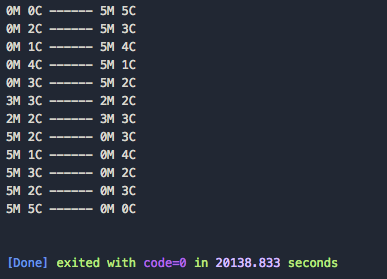
\includegraphics[width=8cm]{resources/mc-3} \\

Después también se actualizó el algoritmo de generación de descendientes para generar solo los nodos válidos, quedando así el resultado de su ejecución, donde se puede observar la mejora en tiempo respecto a la implementación anterior. Si se hubiesen aplicado otras formas de mejora del algoritmo, como una lista de nodos cerrados o una heurística válida, este tiempo debería ser aún menor. \\
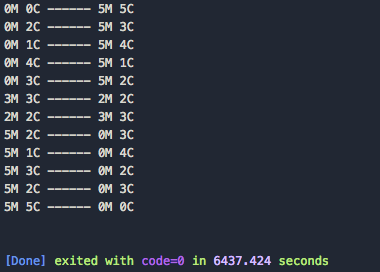
\includegraphics[width=8cm]{resources/mc-3v2} \\


% \begin{thebibliography}{9}
%   \bibitem{c1}
%     Misioneros y Caníbales,
%     \url{https://en.wikipedia.org/wiki/Missionaries_and_cannibals_problem},
%     Wikipedia.
% \end{thebibliography}


\pagebreak
\appendix
\addcontentsline{toc}{section}{\large Anexos}
\noindent\textbf{\huge Anexos}

% para que listings pueda incluir código en español
\lstset{literate=
  {á}{{\'a}}1 {é}{{\'e}}1 {í}{{\'i}}1 {ó}{{\'o}}1 {ú}{{\'u}}1
  {Á}{{\'A}}1 {É}{{\'E}}1 {Í}{{\'I}}1 {Ó}{{\'O}}1 {Ú}{{\'U}}1
  {à}{{\`a}}1 {è}{{\`e}}1 {ì}{{\`i}}1 {ò}{{\`o}}1 {ù}{{\`u}}1
  {À}{{\`A}}1 {È}{{\'E}}1 {Ì}{{\`I}}1 {Ò}{{\`O}}1 {Ù}{{\`U}}1
  {ä}{{\"a}}1 {ë}{{\"e}}1 {ï}{{\"i}}1 {ö}{{\"o}}1 {ü}{{\"u}}1
  {Ä}{{\"A}}1 {Ë}{{\"E}}1 {Ï}{{\"I}}1 {Ö}{{\"O}}1 {Ü}{{\"U}}1
  {â}{{\^a}}1 {ê}{{\^e}}1 {î}{{\^i}}1 {ô}{{\^o}}1 {û}{{\^u}}1
  {Â}{{\^A}}1 {Ê}{{\^E}}1 {Î}{{\^I}}1 {Ô}{{\^O}}1 {Û}{{\^U}}1
  {œ}{{\oe}}1 {Œ}{{\OE}}1 {æ}{{\ae}}1 {Æ}{{\AE}}1 {ß}{{\ss}}1
  {ű}{{\H{u}}}1 {Ű}{{\H{U}}}1 {ő}{{\H{o}}}1 {Ő}{{\H{O}}}1
  {ç}{{\c c}}1 {Ç}{{\c C}}1 {ø}{{\o}}1 {å}{{\r a}}1 {Å}{{\r A}}1
  {€}{{\euro}}1 {£}{{\pounds}}1 {«}{{\guillemotleft}}1
  {»}{{\guillemotright}}1 {ñ}{{\~n}}1 {Ñ}{{\~N}}1 {¿}{{?`}}1
}

\lstset{
  basicstyle=\small\ttfamily,
  language=Lisp,
  keywordstyle=\color{blue}\ttfamily,
  stringstyle=\color{red}\ttfamily,
  commentstyle=\color{gray}\ttfamily
}

\section{Implementación MC-1 en Lisp-Scheme}
\lstinputlisting{code/mc-1.rkt}

\pagebreak
\section{Implementación MC-3 en Lisp-Scheme}
\lstinputlisting{code/mc-3.rkt}

\end{document}